\documentclass[border=6pt]{standalone}
\usepackage{tikz}
\usetikzlibrary{arrows.meta,calc,positioning}
\begin{document}
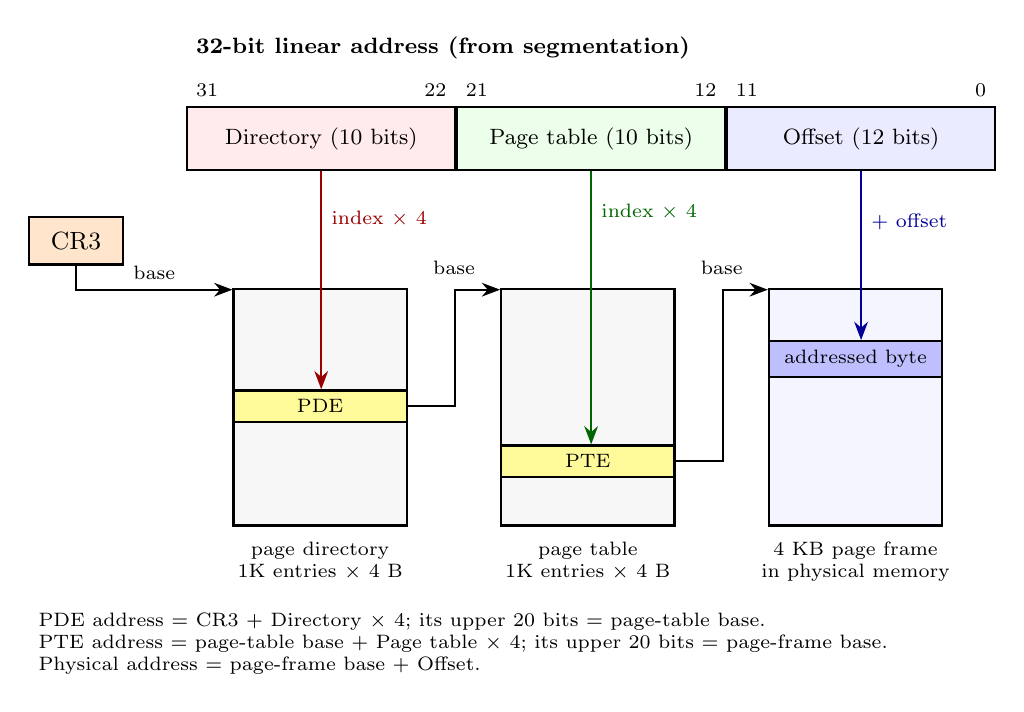
\begin{tikzpicture}[>=Stealth,font=\small,
 fld/.style={draw,thick,minimum height=0.8cm,align=center,font=\footnotesize},
 tbl/.style={draw,thick,minimum width=2.2cm,minimum height=3.0cm,fill=gray!6},
 ent/.style={draw,thick,fill=yellow!40,minimum width=2.2cm,minimum height=0.4cm,font=\scriptsize},
 tcap/.style={font=\scriptsize,align=center,below=2pt}]
% linear address
\node[font=\footnotesize\bfseries,anchor=west] at (0,1.15) {32-bit linear address (from segmentation)};
\node[fld,minimum width=3.4cm,fill=red!8,anchor=west] (dir) at (0,0) {Directory (10 bits)};
\node[fld,minimum width=3.4cm,fill=green!8,right=0pt of dir] (tab) {Page table (10 bits)};
\node[fld,minimum width=3.4cm,fill=blue!8,right=0pt of tab] (off) {Offset (12 bits)};
\node[font=\scriptsize,anchor=south west] at (dir.north west) {31};
\node[font=\scriptsize,anchor=south east] at (dir.north east) {22};
\node[font=\scriptsize,anchor=south west] at (tab.north west) {21};
\node[font=\scriptsize,anchor=south east] at (tab.north east) {12};
\node[font=\scriptsize,anchor=south west] at (off.north west) {11};
\node[font=\scriptsize,anchor=south east] at (off.north east) {0};
% tables, each under its field
\node[tbl,anchor=north] (pd) at (1.7,-1.9) {};
\node[tcap] at (pd.south) {page directory\\1K entries $\times$ 4 B};
\node[ent] (pde) at ($(pd.north)+(0,-1.5)$) {PDE};
\node[tbl,anchor=north] (pt) at (5.1,-1.9) {};
\node[tcap] at (pt.south) {page table\\1K entries $\times$ 4 B};
\node[ent] (pte) at ($(pt.north)+(0,-2.2)$) {PTE};
\node[tbl,anchor=north,fill=blue!4] (pg) at (8.5,-1.9) {};
\node[tcap] at (pg.south) {4 KB page frame\\in physical memory};
\node[ent,fill=blue!25] (byte) at ($(pg.north)+(0,-0.9)$) {addressed byte};
% index arrows (vertical)
\draw[->,thick,red!60!black] (dir.south) -- (dir.south |- pde.north) node[pos=0.22,right,font=\scriptsize]{index $\times$ 4};
\draw[->,thick,green!40!black] (tab.south) -- (tab.south |- pte.north) node[pos=0.15,right,font=\scriptsize]{index $\times$ 4};
\draw[->,thick,blue!60!black] (off.south) -- (off.south |- byte.north) node[pos=0.3,right,font=\scriptsize]{+ offset};
% CR3 gives the directory base
\node[draw,thick,fill=orange!20,minimum width=1.2cm,minimum height=0.6cm] (cr3) at (-1.4,-1.3) {CR3};
\draw[->,thick] (cr3.south) |- ($(pd.north west)+(0,-0.02)$) node[pos=0.75,above,font=\scriptsize]{base};
% chaining: upper 20 bits of an entry = base of the next level
\draw[->,thick] (pde.east) -- ++(0.6,0) |- ($(pt.north west)+(0,-0.02)$);
\draw[->,thick] (pte.east) -- ++(0.6,0) |- ($(pg.north west)+(0,-0.02)$);
\node[font=\scriptsize,anchor=south] at (3.4,-1.85) {base};
\node[font=\scriptsize,anchor=south] at (6.8,-1.85) {base};
\node[font=\scriptsize,align=left,anchor=north west] at (-2.0,-5.9) {PDE address = CR3 + Directory $\times$ 4; its upper 20 bits = page-table base.\\
PTE address = page-table base + Page table $\times$ 4; its upper 20 bits = page-frame base.\\
Physical address = page-frame base + Offset.};
\end{tikzpicture}
\end{document}
